\documentclass[11pt,a4paper,DIV=9]{scrartcl}

\usepackage{tikz}
\usepackage{ngerman}
\usepackage[utf8]{inputenc}
\usepackage{amsmath,amssymb}
\usepackage{hyperref}
\hypersetup{linktoc=all}
% Schriftart ändern
\renewcommand{\rmdefault}{ppl}
%Möglichkeit zur Änderung von Überschriften
\usepackage{sectsty}
%Überschrift \section uandern
\definecolor{blue}{RGB}{76 , 92, 153}
\allsectionsfont{\color{blue}}
\paragraphfont{\color{blue}}

%Variable Blattnummer
\newcommand{\blatt}[1]{
  \newcommand{\blattnr}{#1}
}
%Aufgabe und Aufgabenteil definieren
\newcounter{temp}
\newcommand{\aufgabe}[1]{
  \setcounter{temp}{\value{subsection}}
  \setcounter{subsection}{#1}
  \addtocounter{subsection}{-1}
  \subsection{Aufgabe}
  \setcounter{subsection}{\value{temp}}
}
\newcommand{\teil}[2][]{
  \subsubsection*{#2) #1}
}
\renewcommand{\author}[1]{\renewcommand{\author}{#1}}
\renewcommand{\title}[1]{\renewcommand{\title}{#1}}
\newcommand{\makehomeworktitle}{
  \begin{minipage}[t]{6.5cm}
    \sf{\author}
  \end{minipage}
  \begin{minipage}[t]{6.5cm}
    \begin{flushright}
      \sf{\title\\\today}
    \end{flushright}
  \end{minipage}
  \\[0.2cm]
  \begin{center}
    \sf{
      \color{blue}{
        \LARGE{Dokumentation First.FM}
      }
    }
  \end{center}
  \vspace{0.1cm}
}

%%%%%%%%%%%%%%%%%%%%%%%%
%%% Statisch
\author{{[}4131658{]} Jan Germann \\{[}4054962{]} Christian Ratz\\Übungsgruppe 1}
\title{SQL Praktikum}

%%% Auf jedes Hausaufgabenblatt anpassen
\blatt{1}
%%%%%%%%%%%%%%%%%%%%%%%%
\begin{document}
\makehomeworktitle
\tableofcontents
\newpage
\section{Einleitung}
  \subsection{Allgemeines}
    // TODO Einleitung anpassen.

  \subsection{Formatierung} 
    In der Dokumentation sowie im dazugehörigen Diagramm gilt die folgende Formatierung.

    \begin{description}
      \item [Klassennamen] \hfill \\
        Der Name einer Klasse ist im Regelfall \textbf{fett} formatiert.
      \item [Attribute] \hfill \\
        Attribute einer Klasse sind folgendermaßen gekennzeichnet
        \begin{itemize}
          \item[-] Reguläres Attribut
          \item[*] Attribut ist Teil des Primärschlüssel
          \item[/] Abgeleitetes Attribut
          \item[+] Fremdschlüssel
        \end{itemize}
      \item[Relationentypen] \hfill
      \begin{itemize}
        \item Reguläre Relationen zwischen Klassen sind durch eine einfache schwarze Linie gekennzeichnet.
        \item Sogenannte \textit{XOR}-Relationen besitzen an der ausgehenden Klasse ein Rautesymbol ($\blacklozenge$). Hierbei darf die Klasse, für die gespeicherte Entität, nur mit einer einzigen der Klassen gleichzeitig in Relation stehen.
      \end{itemize}
    \end{description}


\section{Pre-Integration Analyse}
  Bei der Betrachtung der gegebenen Schemata ist zu erkennen, dass es nur wenige Schnittpunkte gibt. Dies erlaubt eine relativ problemlose Zusammenführung beider Schemata.
  Die Schnittpunkte finden sich in den Klassen
  \begin{description}
    \item [\textbf{User} und \textbf{Benutzer}]
    \item \textbf{Comment} und \textbf{Kommentare}
    \item \textbf{Genre} und \textbf{Genres}
  \end{description}

\section{Vergleich der Schemata}
  Beim Verg

\section{Angleichung der Schemata}
  \subsection{Genre}
    Die Klasse \textbf{Genre} wurde um das Attribut -type ergänzt, welches durch einen numerischen Wert angibt, ob es sich dabei um ein Musik- oder Filmgenre handelt.

  \subsection{Comment}
    Die Klasse \textbf{Comment} wurde um das Attribut -update ergängzt. Hiermit wird der Anforderung Sorge getragen, dass auch der eventuelle Änderungszeitpunkt eines Kommentars zeitlich gespeichert werden soll. Dies kann nun als neues Feature auch der Userbase von \textsc{first.fm} bereitgestellt werden.
    
  \subsection{User}
    Das Klassendiagramm von \textsc{netflax} sieht vor, dass für Leih- und Kaufverträge Name, Adresse und Kreditkartennummer des Vertragspartners (\textbf{Benutzer}) gespeichert wird. Für die Zusammenführung war es notwendig dies als optionale Attribute zu \textbf{User} hinzuzufügen.



\section{Zusammenführung und Restrukturierung}


% \section{Ergebnis}
% 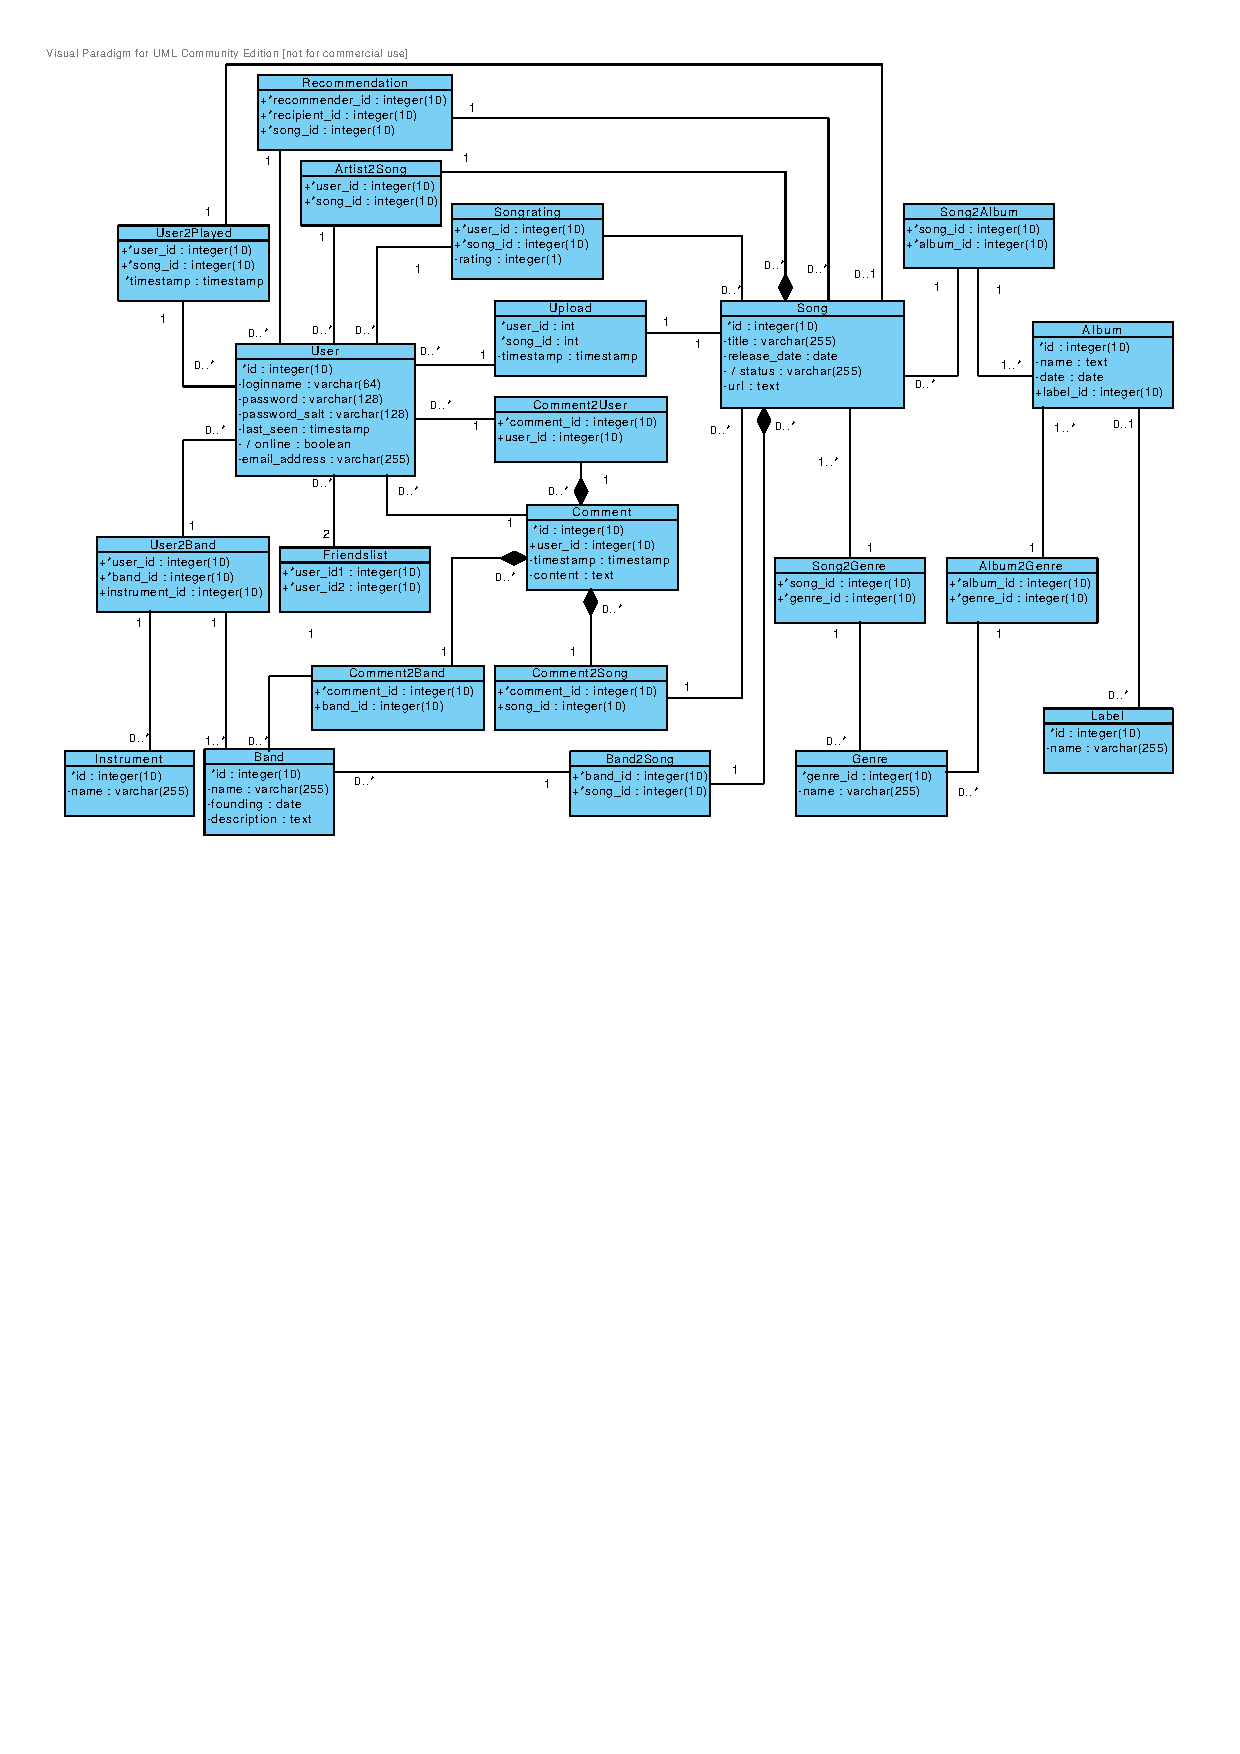
\includegraphics[page=1, angle=90,trim=0cm 0cm 1.1cm 1cm, clip=true, scale=1.1]{Diagram1}
\end{document}